\begin{frame}{Deep CNN}
\begin{itemize}
    \item Histograms and edges are called “shallow” features because we build them by hand
    \item We know we can learn neural network and linear model weights by \textbf{Gradient Descent}
    \item Can we also learn our features?
\end{itemize}
\end{frame}

\begin{frame}{Deep CNN}
\begin{figure}
    \centering
    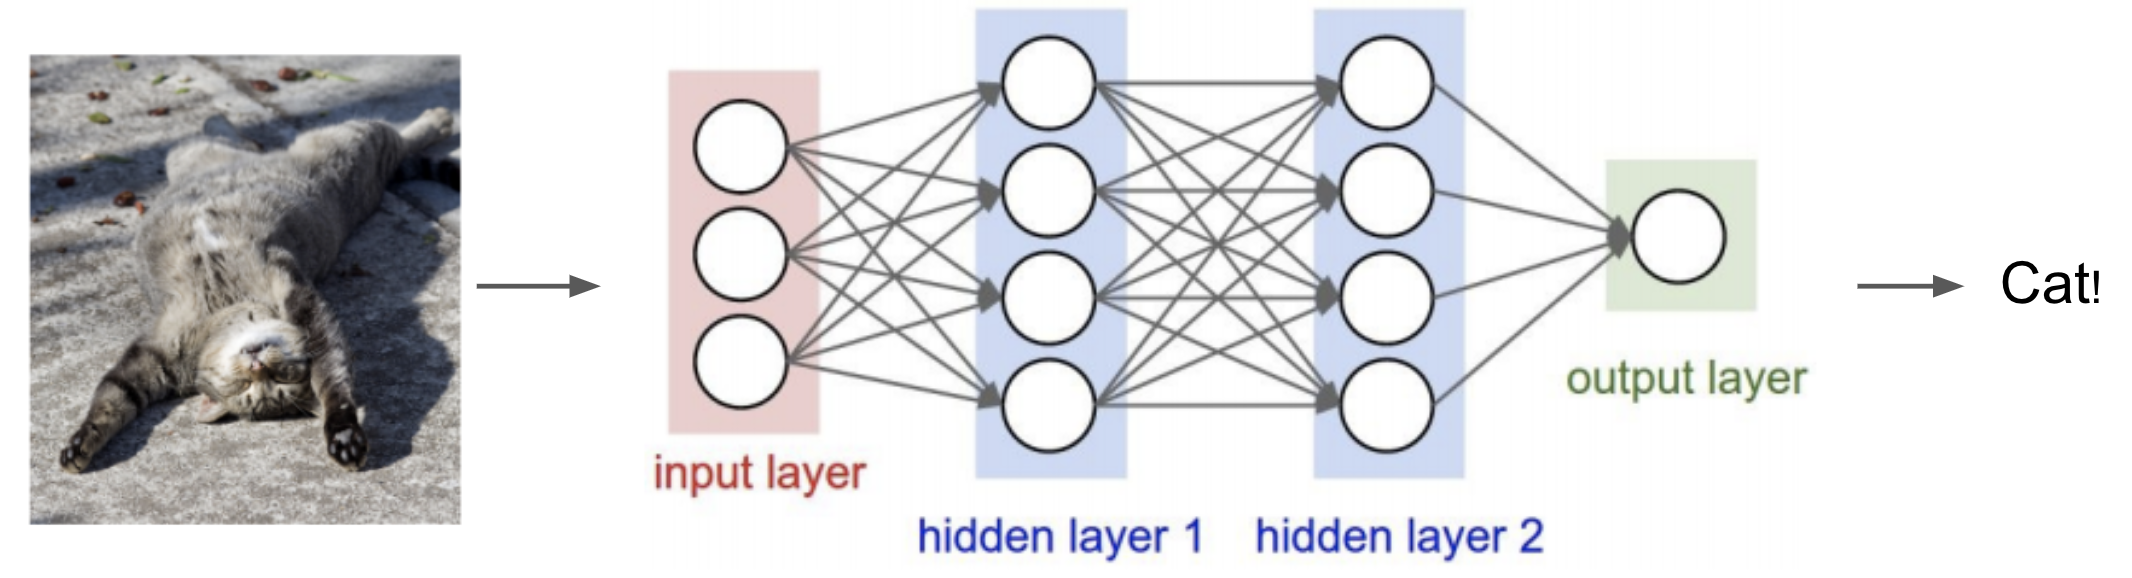
\includegraphics[width=1\textwidth]{img/catNN.png}
    \caption{Our neural network predicting cats must take either flattened cat or extracted features as input.}
\end{figure}
\end{frame}

\begin{frame}{Deep CNN}
\begin{figure}
    \centering
    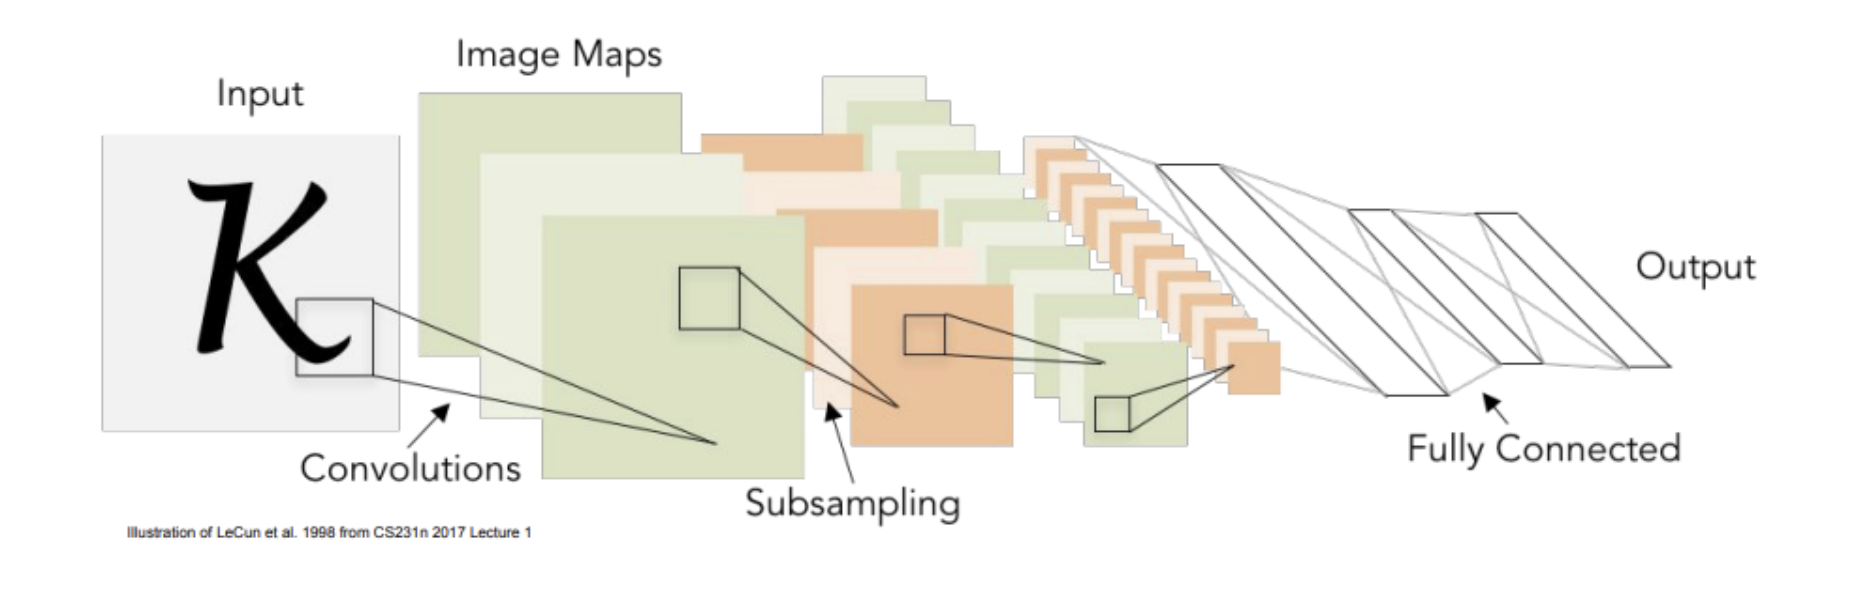
\includegraphics[width=1\textwidth]{img/dcnn.png}
    \caption{In modern Computer Vision, we rely on \textbf{Convolutional Neural Networks} to learn meaningful features by gradient descent.}
\end{figure}
\footnotetext{http://cs231n.stanford.edu/slides/2019/cs231n\_2019\_lecture05.pdf}
\end{frame}

\begin{frame}{Deep CNN}
\begin{figure}
    \centering
    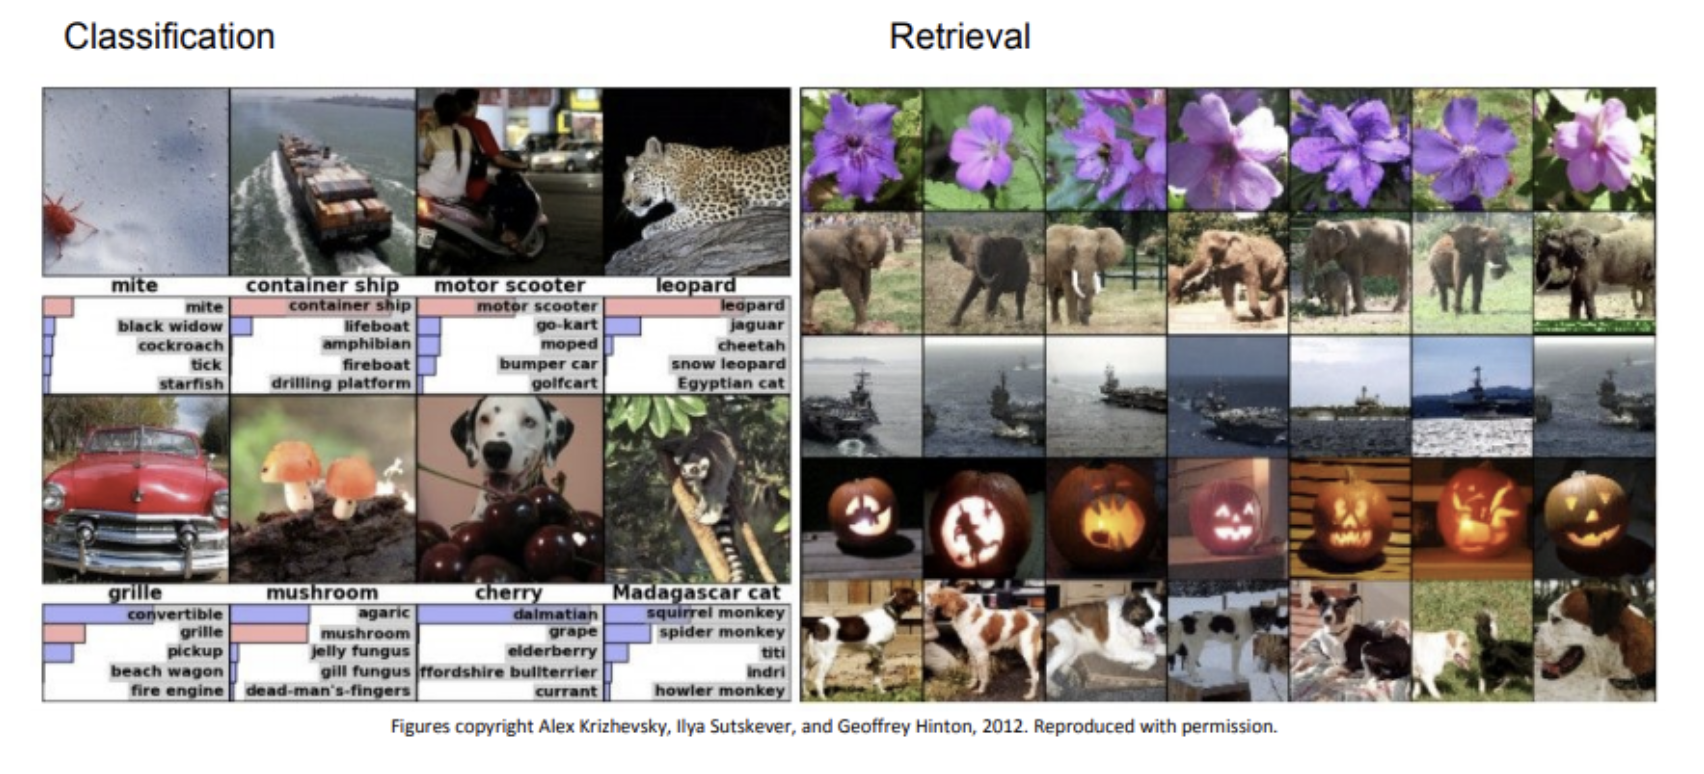
\includegraphics[width=1\textwidth]{img/cnnex1.png}
    \caption{Deep Convolutional Neural Networks are everywhere}
\end{figure}
\footnotetext{http://cs231n.stanford.edu/slides/2019/cs231n\_2019\_lecture05.pdf}

\end{frame}

\begin{frame}{Deep CNN}
\begin{figure}
    \centering
    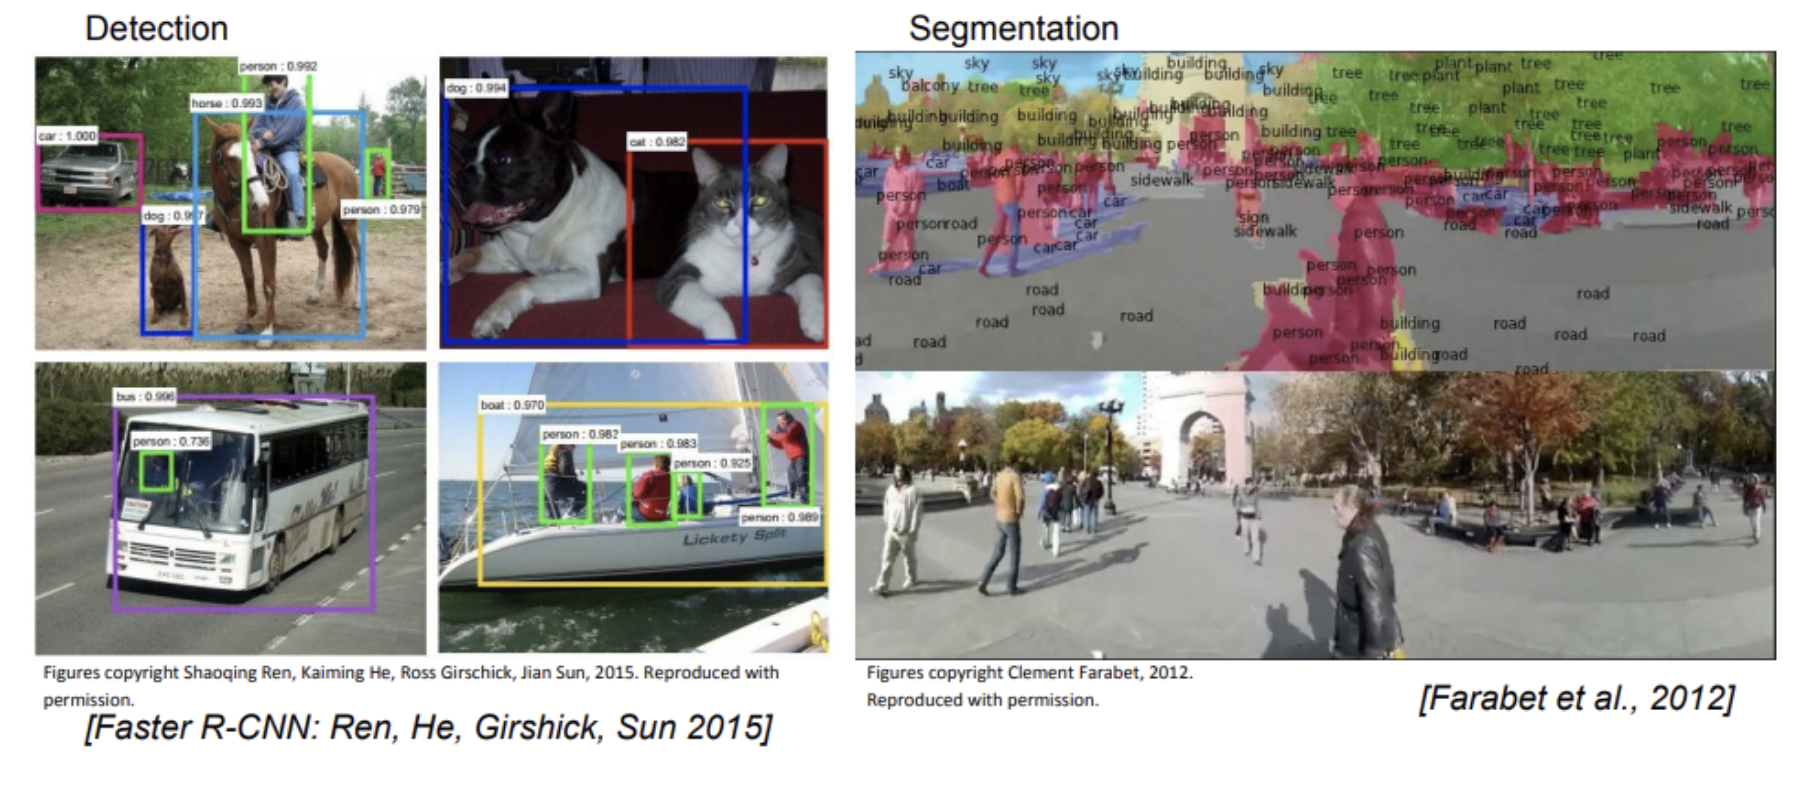
\includegraphics[width=1\textwidth]{img/cnnex2.png}
    \caption{Deep Convolutional Neural Networks are everywhere}
\end{figure}
\footnotetext{http://cs231n.stanford.edu/slides/2019/cs231n\_2019\_lecture05.pdf}
\end{frame}

\begin{frame}{Deep CNN}
\begin{figure}
    \centering
    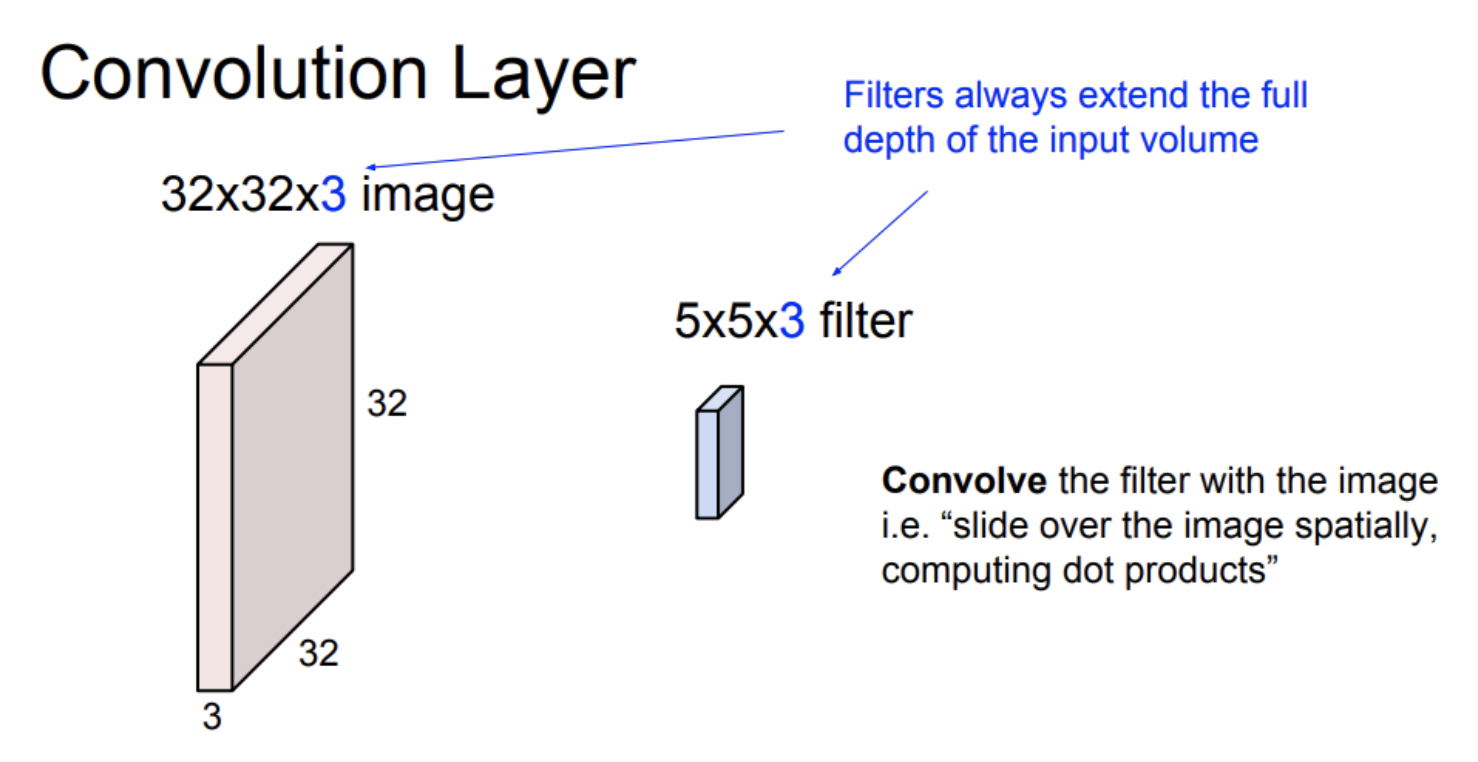
\includegraphics[width=0.8\textwidth]{img/convlayer1.png}
    \caption{Convolutional Layers}
\end{figure}
\footnotetext{http://cs231n.stanford.edu/slides/2019/cs231n\_2019\_lecture05.pdf}
\end{frame}

\begin{frame}{Deep CNN}
\begin{figure}
    \centering
    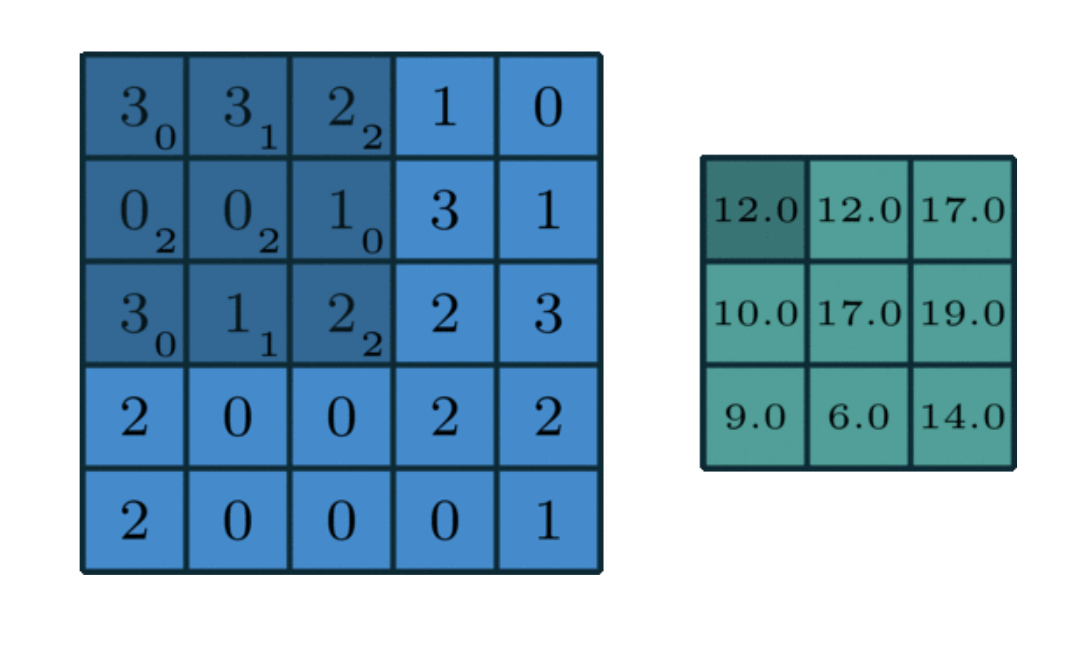
\includegraphics[width=0.8\textwidth]{img/convlayer2.png}
    \caption{Convolutional Layers}
\end{figure}
\end{frame}

\begin{frame}{Deep CNN}
\begin{figure}
    \centering
    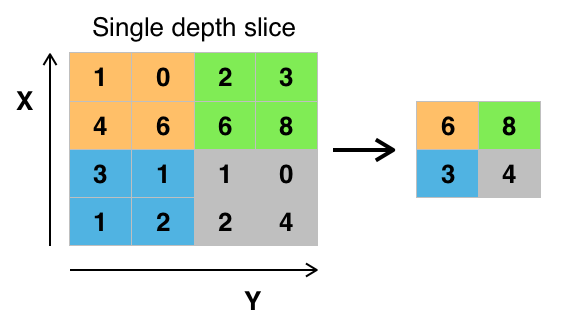
\includegraphics[width=0.8\textwidth]{img/Max_pooling.png}
    \caption{Max Pooling Layers}
\end{figure}
\end{frame}

\begin{frame}{Deep CNN}
\begin{figure}
    \centering
    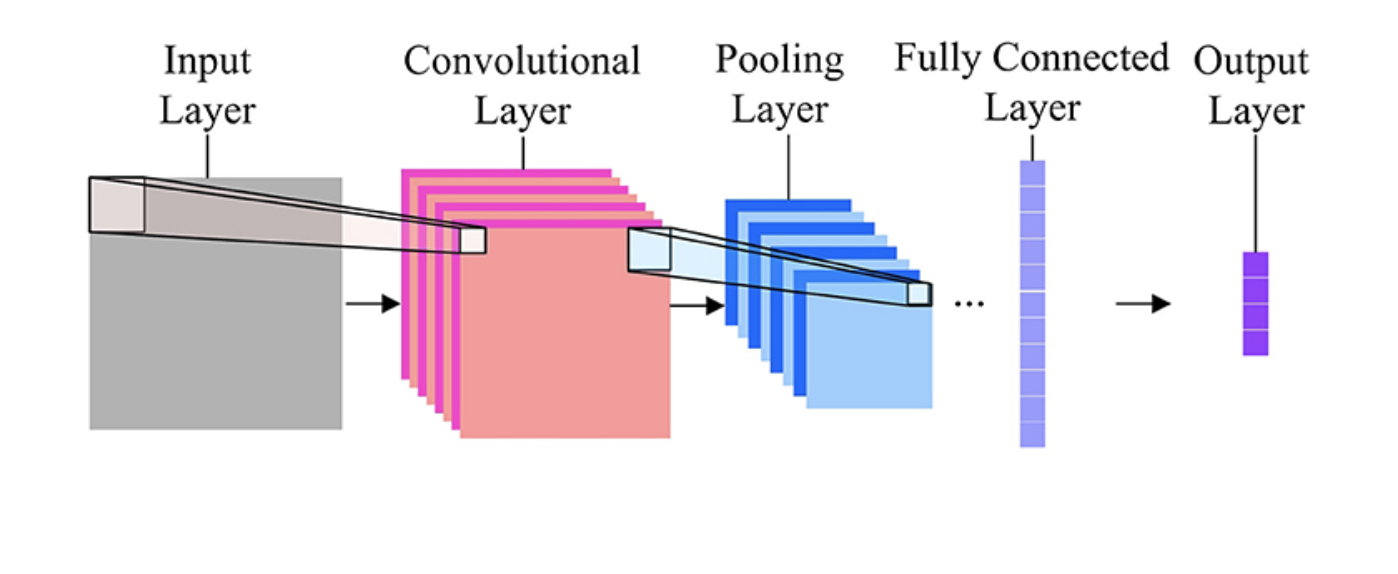
\includegraphics[width=1\textwidth]{img/cnn_structure.png}
    \caption{Full CNN Structure}
\end{figure}
\end{frame}